\section{Experimental Comparison}\label{sec:experimental-comparison}

The three loss functions presented in Section~\ref{sec:loss-functions} were experimentally evaluated on 20 publicly available datasets and on a corporate dataset from the domain of computer security. The 2 metrics presented in Section~\ref{sec:clustering-metrics} were used, i.e. the Silhouette coefficient and the accuracy of a kNN classifier built on the embedding. Both of these metrics were tracked over the learning period to also evaluate how the models are learning in addition to their final performance.

\subsection{Datasets}

The evaluation was done on a set of 20 publicly available datasets. These are, in alphabetical order:
\begin{enumerate}
  \item The "BrownCreeper" and "WinterWren" datasets. See \cite{briggs_rank-loss_2012}. A dataset of bird songs where each bag represents a recording of one or multiple birds. Originally a 13-class dataset, converted to binary classification datasets by selecting a target class.
  \item The "CorelAfrican" and "CorelBeach" datasets. See \cite{chen_miles:_2006}. A dataset of object images where each bag is an image, consisting of segments described by \( 4 \times 4 \) patch features. Originally a 20-class dataset, converted to binary classification datasets by selecting a target class.
  \item The "Elephant", "Fox" and "Tiger" datasets. See \cite{andrews_support_2002}. A dataset of animal images where each bag is an image, consisting of segments. Originally a multi-class dataset (also with animals other that the 3), converted to binary classification datasets by selecting a target class.
  \item The "Musk1" and "Musk2" datasets. See \cite{dietterich_solving_1997}. A dataset of molecules where each bag is a set of the different shapes the molecule can fold into (so-called \textit{conformers}). The goal is to predict whether a molecule has a musky smell or not. If at least one of the conformers of a molecule can cause it to smell musky, the molecule is positive.
  \item The "Mutagenesis1" and "Mutagenesis2" datasets. See \cite{srinivasan_comparing_1995}. A dataset consisting of a drug activity prediction problem. There is an easy ("Mutagenesis1") and a hard ("Mutagenesis2") version.
  \item The "Newsgroups1", "Newsgroups2" and "Newsgroups3" datasets. See \cite{zhou_multi-instance_2008}. A text categorization dataset where each bag is a collection of posts from different newsgroups. A positive bag for a class is designed to contain 3\% of posts from the target class and 97\% randomly sampled from the other categories. Originally a 20-class dataset, converted to binary classification datasets by selecting a target class.
  \item The "Protein" dataset. See \cite{ray_learning_2005} and \cite{ray_supervised_2005}. A dataset consisting of protein annotations making it a text categorization problem. The task is to decide whether a given pair should be annotated by a Gene Ontology (GO) code.
  \item The "UCSBBreastCancer" dataset. See \cite{kandemir_empowering_2014}. A dataset consisting of 38 TMA image excerpts from breast cancer patients where each bag represents an image excerpt consisting of image patches. The goal is to predict whether the cancer is benign or malignant.
  \item The "Web1", "Web2", "Web3" and "Web4" datasets. See \cite{zhou_multi-instance_2005}. A dataset of webpages as ranked by 4 different users based on their being interesting. Each bag represents a webpage with instances being the links on the webpage.
\end{enumerate}

All the datasets as used were made public in \cite{dedic_mildatasetsjl_2019}.

The models were also evaluated on a proprietary dataset provided by Cisco Cognitive Intelligence, consisting of records of network connections from clients (e.g. user computers or mobile devices) to some on-line services. The dataset represents HTTP traffic of more than 100 companies. Two datasets were collected, each spanning 1 day of traffic. The training data was traffic from 2019-11-18, while the data used for testing was collected the following day, 2019-11-19. For each connection, a proprietary classification system based on \cite{jusko_graph-based_2017} provided labels, classifying the connections either as legitimate or malicious (connected to malware activity). The data was sampled to include 90\% of negative bags and 10\% of positive bags. For each connection, 20 connection features were used, as well as a MIL model of the server URL, which is visualized in Figure~\ref{fig:URL-model}.

\begin{figure*}
  \centering
  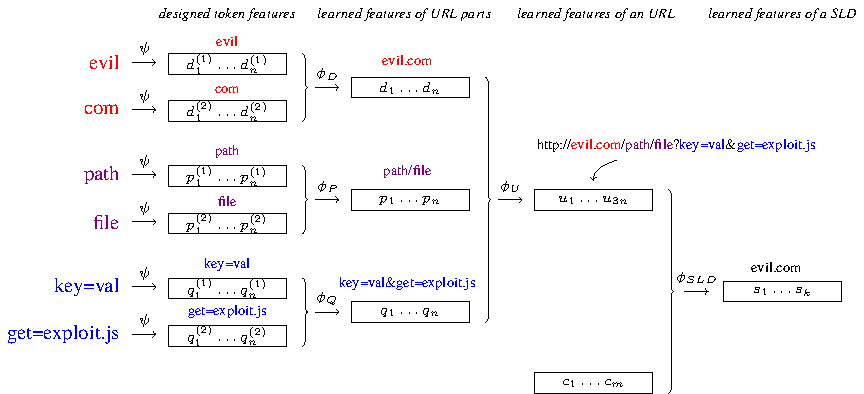
\includegraphics[width=\textwidth]{images/URL-model/URL-model.pdf}
  \caption{Hierarchical model of a URL. The vector \( c_1, \dots, c_m \) represents the connection features.}\label{fig:URL-model}
\end{figure*}

\subsection{Experimental Design}

\subsection{Comparison Results}\label{sec:experiment-comparison}
